\chapter{Implementation}
\label{sec:implementation}

In this chapter, an implementation of the solution suggested in previous chapters is described with usage of UML class diagrams and important code fragments.

\section{Tools Used}

\subsection{Programming language}

The suggested algorithm was implemented in the Java language which is running on the official virtual machine (Oracle JVM version 1.6). The Java language was chosen mainly because of its simplicity and the rich library of collections. A lot of time and debugging was saved by using the built-in functionality, mainly collections. The most used collections include lists, sets and queues. The lists (mainly the {\tt ArrayList} implementations) are often used instead of arrays, but only at places where it is reasonable to do so. For example, an array list has a method to shuffle its elements, which can be useful in certain mutation operations.

As the Java is an interpreted language, many people are concerned about its performance. However, the speed of a well-written program coded in Java is fully comparable with the same program implemented in a low-level machine oriented language, such as {\tt C} or {\tt C++}. Advanced technologies, e.g. the JIT compilation, provide huge possibilities to optimise the bytecode by the virtual machine itself on the fly. Also, the automatic memory management in the Java Virtual Machine offers more pros than cons. Without a programmer managing the memory manually, more time can be invested to the algorithm optimisation. There is a plenty of memory these days and its reasonable usage to take advantage of caching, etc. is often more useful than saving it aimlessly.

\subsection{IDE and plugins}

All the coding was done in the Eclipse IDE (Helios). Tools used for the static code analysis, to ensure the highest code quality, include FindBugs, PMD, CodePro AnalytiX, UCDetector and ECLEmma. Unit tests were prepared using the JUnit test framework. Their code coverage is about 90\%. Most of the remaining 10\% are exceptional states or program paths that should not be reached under the normal circumstances (state checking, I/O exceptions, testing methods). The unused code was mostly deleted, but there is still some remaining in the sake of further debugging or preparing illustrations and tests for the thesis.

Code checking during the development was very strict, there are no warnings in the code (although almost all the checking rules available in the Eclipse IDE were enabled). The motivation was to use as many tools as possible to avoid technical mistakes, dodgy code, dangerous constructions and to keep the best practises through the whole codebase.

\subsection{Coding style and philosophy}

Most of the code is written using a functional approach to prevent state- related bugs and to increase the ability to write accurate unit tests. Most classes are immutable. This style allows the programmer to be less concerned about the internal state of objects. Instead of changing the object's state, a new one is created. As a drawback, more memory is used than necessary, and the garbage collector sweeps the heap more often. However, most of the objects created have a very short lifespan. Therefore, the generational garbage collector in JVM removes them quickly and reclaims a lot of memory for further use quickly.

The code contains a reasonable amount of commentaries in Javadoc. The coding style chosen is is based on C style. It features new line brackets and a lot of whitespace. There was no reason to keep up to a code guide, because the project was primarily aimed as a proof of the concept only. After all, the code formatting is the least important as the most today's IDEs feature an automatic formatter with a lot of style settings.

\section{Architecture Overview}

\begin{table}
\centering
\begin{tabular}{|p{.25\textwidth}|p{.7\textwidth}|}
\hline
{\bf Module} & Basic geometric structures (2D position, 2D rectangle, the module and the placed module). Used for decoding floorplans from their representation and evaluating the result. \\
\hline
{\bf B*-Tree} & The B*-Tree node and related utilities (the placer, the placement evaluator, the node number generator, the node number finder, the prototype generator). Used for the floorplan structure representation. \\
\hline
{\bf POEMS} & The POEMS algorithm, the POEMS actions, their sequences and the genetic algorithm for optimizing them. The heart of the floorplan problem solver. \\
\hline
{\bf Program} & Miscellaneous utilities. Used for running benchmarks, importing and exporting problems and their solutions, the logger, the utility method library and the program configuration. \\
\hline
\end{tabular}
\caption{The main program parts}
\label{tab:parts}
\end{table}

The whole program is composed of four main parts: The {\em Module} (geometry related classes), the {\em B*-Tree} (floorplan related classes), the {\em POEMS} (optimisation algorithm classes) and the {\em Program} (support classes). They are summarized in Table~\ref{tab:parts}. The suggested algorithm basically works as follows. First, the problem is loaded (for example, a benchmark) and the prototype solution is generated. Then, this prototype solution is optimised in iterations by the POEMS algorithm \cite{poems} that uses the internal genetic algorithm for local search, that is for finding the best modification of the prototype. After each iteration, the prototype is either replaced by the improvement or kept untouched as it is, whichever is better. After the specified number of iterations, the algorithm ends and outputs the improved prototype. 

The general overview schema is shown in Fig.~\ref{fig:overview} and the pseudocode in Fig.~\ref{fig:algorithm}. The individual steps will be described in more detail in the following chapters.

\begin{figure}
\centering
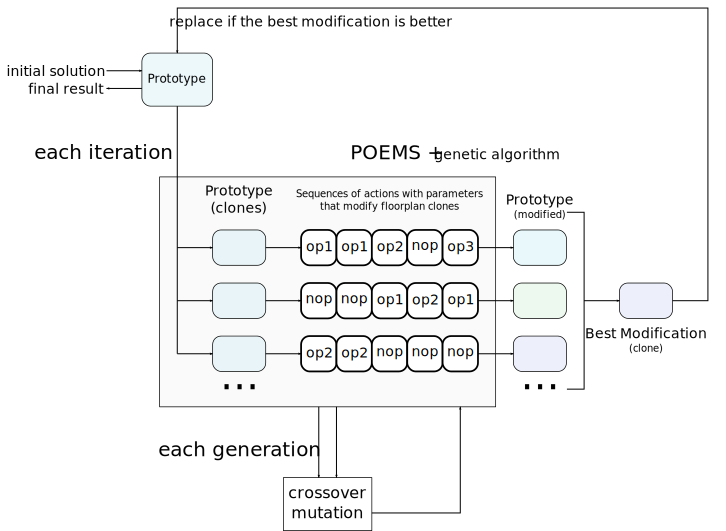
\includegraphics[width=\textwidth]{algorithm}
\caption{Overall program schema}
\label{fig:overview}
\end{figure}

\begin{figure}
\centering
\begin{algorithmic}[1]
  \STATE{create a new B*-Tree prototype $ \beta $}
  \FOR{$ i $ in range 1 .. $ i_\mathrm{max} $}
    \STATE{sequence $ S_\mathrm{best} $ = (unset)}
    \STATE{create a random population of sequences}
    \FOR{$ g $ in range 1 .. $ g_\mathrm{max} $}
      \IF{random real number $ \in \langle 0, 1) < P_\mathrm{crossover} $}
        \STATE{select two parents $ P_1, P_2 $ by applying the selection operator}
        \STATE{create two descendants $ C_1, C_2 $ using the crossover operator on $ P_1, P_2 $}
        \STATE{insert both individuals $ C_1, C_2 $ into the population}
      \ELSE
        \STATE{select one individual $ M $ by applying the selection operator}
        \STATE{create descendant $ C $ by using the mutation operator on $ M $}
        \STATE{insert the individual $ C $ into the population}
      \ENDIF
      \STATE{sequence $ S_\mathrm{temp} $ = the best sequence in the population}
      \IF{the fitness of $ S $ is better than the fitness of $ S_\mathrm{best} $}
        \STATE{$ S_\mathrm{best} = S_\mathrm{temp} $}
      \ENDIF
    \ENDFOR
    \IF{the fitness of $ S_\mathrm{best} $ is better or equal to the fitness of $ \beta $}
      \STATE{$ \beta $ = $ \beta $ modified by sequence $ S_\mathrm{best} $}
    \ENDIF
  \ENDFOR
  \RETURN{$ \beta $}
\end{algorithmic}
\caption{Overall program pseudocode}
\label{fig:algorithm}
\end{figure}

\section{Classes}

This chapter describes important classes and algorithms used in the algorithm suggested. The language in which the algorithms are presented here is not exactly the Java, but it is very similar. The main purpose of the code is to provide a low-level view on algorithms and data structures used, and any programmer should be able to understand them and re-implement them in any programming language he or she controls.

The classes are divided into the same groups, as described in the previous section. These groups are the {\em Module} (geometry related classes), the {\em B*-Tree} (floorplan related classes), the {\em POEMS} (optimisation algorithm classes) and the {\em Program} (support classes). Each group contains more Java packages, but these details are unimportant for understanding the algorithm and they are used for developer's convenience only.

\subsection{Module classes}

As the problem solved includes placing rectangles on a plane, some classes representing simple geometric objects must be created: the position is a tuple of 2D coordinates $(X, Y)$ in a 2D Cartesian space. A rectangle is defined by its width and height. The module is a named rectangle, because the name helps identify the module. The placed module is a tuple of a module and its position. 

Each module is unoriented. It means that it can be rotated freely. The rotation here means flipping the width and the height dimensions. For example, the module $A(1, 4)$ rotated is the module $A(4, 1)$. Therefore, a module must be able to rotate with its identity preserved.

The {\tt Position} class is just a tuple of two coordinates $(X, Y)$. This class is used to hold the position of a placed module. The class is immutable.

The {\tt Rectangle} class specifies the width and the height of a rectangle. The class is immutable.

The {\tt Module} class extends the {\tt Rectangle} class, adds a name, a Boolean flip flag and ability to flip the width and height. The flipping operation creates a new instance with dimensions swapped. The class is immutable.

The {\tt PlacedModule} class aggregates the {\tt Module} and the {\tt Position} classes. Each instance represents the module placed at a certain position. The class is immutable.

The class diagram of this part of the algorithm is shown in Fig.~\ref{fig:uml:module}.

\begin{figure}
\centering
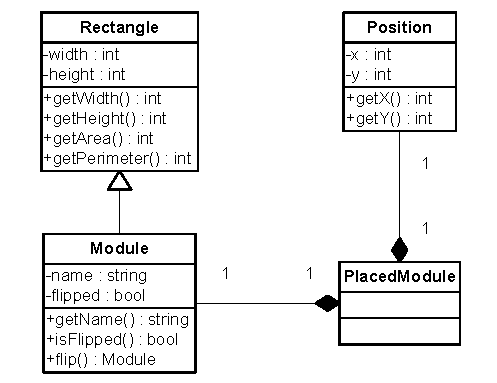
\includegraphics[width=.5\textwidth,page=1]{class}
\caption{Module related classes}
\label{fig:uml:module}
\end{figure}

\subsection{B*-Tree classes}

The B*-Tree is a special kind of a binary tree. Each B*-Tree node carries a value representing exactly one module (unplaced / placed, not numbered / numbered).

The generic {\tt BTree} class represents a B*-Tree node with a value. Each node can be viewed at as a subtree, as a tree is defined recursively as a node or a parent node with child nodes. Each node instance can carry any value implementing the {\tt BTreeValue} interface. These are the {\tt Module}, the {\tt PlacedModule} and the {\tt NumberedValue}. The class is immutable.

The {\tt NumberedValue} class represents a special container for other B*-Tree value providing a tree-wide unique number for identification. This number is used as a node address in POEMS actions. The class is immutable.

The numbers are generated recursively using a {\tt Counter} class used as a `hot potato' which increments its value while visiting nodes. The last value of the counter is needed for limiting random values of POEMS actions.

The class diagram of this part of the algorithm is shown in Fig.~\ref{fig:uml:btree}.

\begin{figure}
\centering
\includegraphics[width=\textwidth,page=2]{class}
\caption{B*-Tree related classes}
\label{fig:uml:btree}
\end{figure}

\subsubsection{B*-Tree placer}

The B*-Tree {\tt Placer} class is used for assigning exact 2D position to each module based on the structure of the given B*-Tree. The rules for this placement are described in previous chapters. The important thing to mention here is, that a special structure is used here to speedup the placement. 

The speedup structure {\tt PlacerCache} is basically is a queue of instances of the {\tt PlacerCacheItem} class which are automatically sorted by their $\mathrm{level}$ property, descending. The $\mathrm{level}$ has the meaning of the top-most $y$ coordinate $\mathrm{position}$ and $\mathrm{width}$ specify the area in which the level is raised.

When placing a module, its $x$ coordinate is given by the node's parent and $y$ depends on items in the queue. The queue is walked from the beginning until a first overlapping item is reached (if none, $0$ is returned). Then, this item's $\mathrm{level}$ coordinate is used as the $y$ coordinate of the newly placed module. Finally, the queue is updated - the level is raised where the new module was placed.

As the queue is not walked whole in most situations, the speedup is significant. The placer performance is evaluated in Table~\ref{tab:placer}.

The class diagram of this part of the algorithm is shown in Fig.~\ref{fig:uml:placer}.

\begin{figure}
\centering
\includegraphics[width=\textwidth,page=3]{class}
\caption{B*-Tree placer related classes}
\label{fig:uml:placer}
\end{figure}

\subsubsection{B*-Tree evaluation}

The quality of each floorplan must be evaluated as it is used as the fitness function in the genetic algorithm. The value measured in this implementation is the amount of the unused area ($S_{\mathrm{unused}}$). For the computation of this value, the total area ($S_{\mathrm{total}}$) and the used area ($S_{\mathrm{used}}$) must be known. 

The total area of the floorplan ($S_{\mathrm{total}}$) is defined as an area of the smallest enclosing rectangle which contains all placed modules in that floorplan. The used area of the floorplan ($S_{\mathrm{used}}$) is defined as a sum of areas of all modules placed in that floorplan. 

The unused area ($S_{\mathrm{unused}}$) is then computed as the $ S_{\mathrm{total}} - S_{\mathrm{used}}$. The fitness of the floorplan is a negative value of the unused area and must be maximized (to minimize the area unused).

On the other hand, the computation of the unused area {\em percentage} ($d$) is not so clear. Various equations are used in the articles, but the most common formula seems to be $d = S_{\mathrm{total}} / S_{\mathrm{used}} - 1 $ (ratio of the unused area and the used area). The same formula is used in the proposed algorithm. An alternative formula is, for example, $d_2 = S_{\mathrm{unused}} / S_{\mathrm{total}}$.

The computation is done by the {\tt Evaluator} utility class and it is stored in an immutable instance of the {\tt Evaluation} class.

\subsection{POEMS classes}

The POEMS algorithm is an iterative algorithm which can be viewed as an optimisation framework. There is an initial solution called the {\em prototype}, which is iteratively optimised by sequences of actions. These sequences can be optimised by any optimisation method. In this work, a genetic algorithm is used because of the good past author's experience in this area. 

Main optimisation algorithm is contained in the {\tt Poems} class. In each iteration, a new instance of the {\tt Population} class is created. Then, the genetic algorithm is started in that class, and the solution is found. If the solution is of better or equal fitness as the prototype, the prototype is replaced.

The class diagram of this part of the algorithm is shown in Fig.~\ref{fig:uml:poems}. The code of the main POEMS engine is written in Fig.~\ref{alg:poems}.

\begin{figure}
\centering
\begin{lstlisting}
Individual solve(Set<Module> modules) {
  // create the prototype
  Individual prototype = createPrototype(modules);
  
  for (int i = 0; i < MAX_ITERATIONS; i++) {
    // ITERATION #i
    // create a new population
    Population population = new Population(prototype);
    // start evolution
    Individual temp = population.runGeneticAlgorithm();
    // replace prototype if a better or equal solution found
    if (temp.isBetterOrEqual(prototype)) {
      prototype = temp;
    }
  }
  
  return prototype;
}
\end{lstlisting}
\caption{Main POEMS algorithm code}
\label{alg:poems}
\end{figure}

\subsubsection{Complete tree heuristic prototype generator}

The algorithm used for building of the prototype B*-tree is based on the well-known array based heap representation. Given a sufficiently long array indexed from $0$, the subtree on index $i$ has its left child located on index $2i+1$ and right child on index $2i+2$. The subtree on index $0$ is considered to be the root. 

The input array of the modules is created from an (unordered) set of modules so they are first rotated to be wider than taller, and then they are sorted by width descending and the height ascending. 

This simple method creates a tree in a linear time. The code of the algorithm is shown in Fig.~\ref{alg:complete}.

\begin{figure}
\centering
\begin{lstlisting}
BTree<Module> createCompleteTree(Set<Module> modules) {
  final Module[] array = new Module[modules.size()];
  // flip modules to be wider than taller and convert to array
  makeModulesWider(modules).toArray(heap);
  // sort the array by width descending, height ascending
  Arrays.sort(array, MODULE_COMPARATOR);
  // create the complete tree recursively
  return Prototyper.createFromArray(array, 0);
}
  
BTree<Module> createFromArray(Module[] input, int index) {
  if (index >= input.length) {
    return null;
  }
    
  return new BTree<Module>(
    input[index],
    createFromArray(input, 2 * index + 1),
    createFromArray(input, 2 * index + 2)
  );
}
\end{lstlisting}
\caption{Creating a complete tree from a module set}
\label{alg:complete}
\end{figure}

\subsubsection{Best-fit heuristic prototype generator}

Another algorithm used for building of the prototype B*-tree is based on the best-fit heuristic. First, the queue of unplaced modules is created from an (unordered) set of modules. They are first rotated to be wider than taller and then they are sorted by the width descending and the height ascending. At the beginning, the empty space to be filled equals the width of the widest module or the square root of the area of all modules, whichever is greater.

While the queue of the unplaced modules is not empty, the `best' module is picked from the queue (that is, the module as close to the queue top as possible) that fits into the current empty space (module width $\leq$ space width). After placing the module, the space is shortened by the module width. If no such module is found, a new level is created and the space is initialized to the default value.

At the same time, a tree is being built. When placing a module {\em next} to the previous one in the same level, it is saved as the left child of the corresponding tree node. When placing a module {\em on top} of the previous one (that is, when ), it is saved as the right child of the corresponding tree node. Therefore, the heuristic must remember the first node placed in the current level. This first node will be extended by the right child when no module fits in the space remaining on the level and a new level must be created. 

This heuristic allows prototypes to be generated in quadratic time. The code of the algorithm is shown in Fig.~\ref{alg:bestfit}.

\begin{figure}
\centering
\begin{lstlisting}
BTree<Module> createBestFit(Set<Module> modules) {
  final Queue<Module> unplaced = createQueue(
    makeModulesWider(modules), 
    MODULE_COMPARATOR
  );
    
  final int defaultSpace = getWidthApproximation(unplaced);
  boolean newLevel = false;
  int space = defaultSpace;
  TempBTree root = null;
  TempBTree current = null;
  TempBTree firstOnLevel = null;
  
  while (!unplaced.isEmpty()) {
    final Module module = pollBestFit(unplaced, space);
    
    if (module == null) {
      // start new level
      space = defaultSpace;
      nextLevel = true;
      continue;
    }
    
    final TempBTree newNode = new TempBTree(module);
    
    if (root == null) {
      root = newNode;
      current = newNode;
      firstOnLevel = newNode;
    } else {
      if (newLevel) {
        firstOnLevel.right = newNode;
        firstOnLevel = newNode;        
        newLevel = false;
      } else {
        current.left = newNode;
      }
      
      current = newNode;
    }
    
    space -= module.getWidth();
  }
  
  return convertToBTree(root);
}
\end{lstlisting}
\caption{Creating a tree from a module set by the best-fit heuristic}
\label{alg:bestfit}
\end{figure}

\begin{figure}
\centering
\begin{lstlisting}
Module pollBestFit(Queue<Module> unplaced, int space) {
  for (final Module module : unplaced) {
    if (module.getWidth() <= space) {
      // first feasible module found in the queue
      unplaced.remove(module);
      return module;
    }
  }
  
  return null;
}
\end{lstlisting}
\caption{Finding the `best' module to fit into the space provided}
\label{alg:bestfittree}
\end{figure}

\subsubsection{POEMS actions}

There are 6 actions in the POEMS algorithm, and proper implementation of these actions was the most difficult part of the development of the suggested algorithm. The code is too long to be shown here, but it is mostly based on one recursive function that processes the input tree and modifies it at certain places, the rest of the tree is copied without any change (because the trees are immutable and each change results in creating new instances).

All actions have 1, 2 or 3 parameters. The parameter types include {\bf integer} and {\bf Boolean}. The integer parameters specify the B*-Tree node number (an unique address of the node), while the Boolean parameters modify the behaviour of the action. All actions further include a Boolean flag that specifies if the action is enabled or disabled. Disabled actions do not modify the tree at all, so they can be skipped. 

The {\tt PoemsActionSequence} class represents a sequence of actions, applied one after another. It is an fixed-length array of instances of the {\tt AbstractPoemsAction} class, which is the abstract base class for all actions. The length of the sequence can be specified with the problem set and it is fixed during the whole run. The number of enabled actions in the sequence is called the sequence {\em niché}. Each individual in the population holds exactly one sequence of actions. 

Finally, the individual POEMS actions are represented by the following classes. All action classes including the action sequence are immutable.

\begin{itemize}
\item{{\tt FlipPoemsAction}}
\item{{\tt RotatePoemsAction}}
\item{{\tt MirrorPoemsAction}}
\item{{\tt ExchangeNodePoemsAction}}
\item{{\tt ExchangeValuePoemsAction}}
\item{{\tt HangNodePoemsAction}}
\end{itemize}

\subsubsection{Genetic algorithm}

The steady-state genetic algorithm was used because fast convergence is preferred. The code of the genetic algorithm is included in the {\tt Population} class. 

The population consists of several {\em nichés} - groups with the same minimal amount of enabled actions. Initially, each niché contains the same amount of individuals which are generated randomly. The population is represented as an array of individuals. Each niché number $n$ takes a continuous, single and unambiguous range of indices $\langle (n-1) \cdot s, n \cdot s - 1 \rangle$, where the $s$ is the niché size (count of individuals in each niché). In each niché $n$, there are only individuals with $n$ or more enabled actions. 

\begin{figure}
\centering
\subfloat[initial population]{
\begin{tabular}{|r|l|l|}
\hline
Index & Niché & Individual \\
\hline
\hline
0 & 1 & $ \blacksquare \Box \Box \Box $ \\
1 & 1 & $ \Box \Box \blacksquare \Box $ \\
2 & 1 & $ \blacksquare \Box \Box \Box $ \\
\hline
3 & 2 & $ \blacksquare \Box \Box \blacksquare $ \\
4 & 2 & $ \Box \Box \blacksquare \blacksquare $ \\
5 & 2 & $ \Box \blacksquare \Box \blacksquare $ \\
\hline
6 & 3 & $ \blacksquare \blacksquare \blacksquare \Box $ \\
7 & 3 & $ \Box \blacksquare \blacksquare \blacksquare $ \\
8 & 3 & $ \blacksquare \blacksquare \Box \blacksquare $ \\
\hline
9 & 4 & $ \blacksquare \blacksquare \blacksquare \blacksquare $ \\
10 & 4 & $ \blacksquare \blacksquare \blacksquare \blacksquare $ \\
11 & 4 & $ \blacksquare \blacksquare \blacksquare \blacksquare $ \\
\hline
\end{tabular}
} \hspace{1em}
\subfloat[population later]{
\begin{tabular}{|r|l|l|}
\hline
Index & Niché & Individual \\
\hline
\hline
0 & 1 & $ \blacksquare \Box \blacksquare \Box $ \\
1 & 1 & $ \Box \blacksquare \blacksquare \Box $ \\
2 & 1 & $ \blacksquare \blacksquare \blacksquare \Box $ \\
\hline
3 & 2 & $ \blacksquare \Box \Box \blacksquare $ \\
4 & 2 & $ \blacksquare \blacksquare \Box \blacksquare $ \\
5 & 2 & $ \blacksquare \Box \Box \blacksquare $ \\
\hline
6 & 3 & $ \blacksquare \Box \blacksquare \blacksquare $ \\
7 & 3 & $ \blacksquare \blacksquare \blacksquare \blacksquare $ \\
8 & 3 & $ \blacksquare \blacksquare \blacksquare \blacksquare $ \\
\hline
9 & 4 & $ \blacksquare \blacksquare \blacksquare \blacksquare $ \\
10 & 4 & $ \blacksquare \blacksquare \blacksquare \blacksquare $ \\
11 & 4 & $ \blacksquare \blacksquare \blacksquare \blacksquare $ \\
\hline
\end{tabular}
}
\caption{A population with 4 nichés of size 3}
\label{fig:population}
\end{figure}

This structure allows effective searching for individuals with a minimal number of enabled actions. Example population arrays are shown in Fig.~\ref{fig:population}, where the filled square ($\blacksquare$) represents an enabled action and the empty square ($\Box$) represents a disabled action.

Each individual is represented by an instance of the {\tt Individual} class, which aggregates the B*-Tree of the current prototype and the sequence of the actions that modifies it. The fitness of the individual equals to the fitness of the floorplan that is created by applying the action sequence to the aggregated prototype. In the implementation, the fitness equals to the negative unused area of the floorplan that is created by applying individual's action sequence to the prototype it owns. The class is immutable so the fitness function value is computed exactly once for each individual.

Most of the genetic algorithm is implemented as usual, but several standard operators had to be altered to work with nichés.

A tournament selection with two competitors was chosen. Both competitors, however, must be taken from the same niché. The better of these two individuals is returned in 95\% cases, the other one in 5\% cases. This is an improvement suggested by Goldberg and Deb in \cite{tournament}. The code is shown in Fig.~\ref{alg:selection}. The complexity of the selection algorithm is $O(1)$.

The uniform crossover operator is used, because it is simple and fast to implement, the order of the actions in the sequence does not matter much, and the operator allows any possible combination of the parent's sequences to be created. The complexity of the crossover operator is $O(N)$, where $N$ is the action sequence length.

Various mutation operators are used. These operators are chosen and applied randomly and include the action sequence shuffle, the action type change, the action parameter change and the flipping of the action enabled flag. The complexity of the mutation algorithm is $O(N)$ in the worst case. Probabilities are defined so that small changes are applied more often than big changes.

After the crossover or the mutation operator is applied, the new individual is inserted into the population by means of a special method, shown in Fig.~\ref{alg:accept}. The rules for the replacement are stated as follows. If the new individual has no enabled action, a random individual is created instead. The rest is the same. The new individual replaces the individual which has worse or equal fitness and less or equal count of enabled actions. First such individual is replaced. If no such individual is found the new individual is thrown away.

\begin{figure}
\centering
\includegraphics[width=\textwidth,page=4]{class}
\caption{POEMS related classes}
\label{fig:uml:poems}
\end{figure}

\begin{figure}
\centering
\begin{lstlisting}
void createPopulation() {
  int index = 0;

  for (int niche = 1; niche <= NICHE_COUNT; niche++) {
    for (int i = 0; i < NICHE_SIZE; i++) {
      // create a random individual
      // n = niche (number of enabled actions)
      // i = number of individual in the niche
      population[index++] = randomIndividualForNiche(niche);
    }
  }
}
\end{lstlisting}
\caption{Population creation code}
\label{alg:create}
\end{figure}

\begin{figure}
\centering
\begin{lstlisting}
Individual runGeneticAlgorithm(Individual prototype) {
  Individual best = null;

  for (int g = 0; g < MAX_GENERATIONS; g++) {
    // GENERATION #g
    // pick random niche and boundary indices
    int rand_niche = random(1, NICHE_COUNT);
    int i_low = getNicheLow(rand_niche, NICHE_SIZE);
    int i_high = getNicheHigh(rand_niche, NICHE_SIZE);
    
    if (Math.rand() < P_CROSSOVER) {
      // perform CROSSOVER
      IndividualPair children = doCrossover(select(i_low, i_high), select(i_low, i_high));
      accept(children.getFirst());
      accept(children.getSecond());
    } else {
      // perform MUTATION
      Individual child = doMutation(select(i_low, i_high));
      accept(child);
    }
    
    // update best individual
    best = findBest();
  }
  
  return best;
}
\end{lstlisting}
\caption{Main genetic algorithm code}
\label{alg:genetic}
\end{figure}

\begin{figure}
\centering
\begin{lstlisting}
Individual select(int i_low, int i_high) {
  // pick two random individuals
  Individual a = population[random(i_low, i_high)];
  Individual b = population[random(i_low, i_high)];
  // return better one in 95% cases, worse one in 5% cases
  if (a.isBetter(b)) {
    return (Math.random() < 0.95) ? a : b;
  } else if (b.isBetter(a)) {
    return (Math.random() < 0.95) ? b : a;
  } else {
    // a tie, return random one
    return (Math.random() < 0.5) ? a : b;
  }
}
\end{lstlisting}
\caption{Selection mechanism code}
\label{alg:selection}
\end{figure}

\begin{figure}
\centering
\begin{lstlisting}
void accept(Individual fresh) {
  if (fresh.getNiche() == 0) {
    // no individual can be in niche 0 as there is none
    // so create a random one with at least 1 action enabled
    fresh = Individual.random(random(1, NICHE_COUNT));
  } 
  
  for (int i = 0; i <= getNicheHigh(fresh.getNiche(), NICHE_SIZE); i++) {
    if (population[i].isWorseOrEqual(fresh)) {
      // replace individual at index 'i' and break
      population[i] = fresh;
      break;
    }
  }
}
\end{lstlisting}
\caption{Accepting a new individual algorithm code}
\label{alg:accept}
\end{figure}

\subsection{Program utility classes}

Every program needs to interact with the outside world. The program must be able to load benchmark data from files and export final results in different formats. The floorplan structure is needed to be exported as the DOT script \footnote{DOT is a simple language used for graph visualization} and the placed floorplan as the SVG image \footnote{Scalable Vector Graphics (SVG) is the graphics format maintained by W3C}. For testing purposes, exporting various statistical data, such as GNUPlot \footnote{GNUPlot is a tool for drawing charts by simple scripts} scripts, is very useful.

Several utilities were implemented for use within the program. Important classes for loading and saving problems and their solutions are the {\tt Importer} and the {\tt Exporter}. They provide the functionality to work with benchmark and the SVG, the DOT and the GNUPlot files. In addition, they can also export various statistical data used for comparing the algorithms in the next chapter.

The utility classes include the {\tt Numberator} which takes the B*-Tree and creates the same tree with all nodes numbered, the {\tt Finder} which finds the node by its number, the {\tt Evaluator} which takes the B*-Tree with placed modules and evaluates its quality, and the {\tt Prototyper} which creates prototypes for the POEMS algorithm.

There are even more classes used as a service through the program, such as the {\tt Logger} (gathering program events, debugging), the {\tt Setup} (holds various algorithm probabilities) and the {\tt Utility} (generating the random numbers and Booleans).
